When a model is run on some input, it predicts some output $\hat{y}$, which the model wants to evaluate against the desired value $y$. This evaluation happens, with some error function. This error functions outputs some loss-value which is dependent on how much $\hat{y}$ deviates from $y$. The greater the deviation is, the greater the loss/cost will become.
Based on the size of the loss, the models know with how great magnitude it has to adjust its parameters (weights and biases). The goal is to adjust the parameters, so the predicted output $\hat{y}$, gets as close to the desired output $y$.\\

\noindent
Trying every single combination of weights, in the pursuit of finding the best fitting weights for a specific problem, is a very comprehensive task, even for a computer. This problem is being solved with backpropagation. The idea is to find the minimum value of which the loss function can take. Calculating the gradient is a very effective way of finding this minimum. Finding this minimum can be achieved with various gradient descent algorithms. The gradient describes the slope of the function at a specific point in the graph. Assuming we have a function $f$, the following gradient of this function is $f'$. If $f'$ takes some input x, and $f'(x)$ yields a negative result, it means that the graph currently has a negative slop at this current point. Thus, to get closer to a minimum, we have to increase the value of x. \\

\noindent
But a gradient descent algorithm is an algorithm that finds the minimum given it has a gradient available, it is not the algorithm for finding the gradient. Backpropagation is the method of computing the magnitude each weights gradient has on the final error. The way this is done is by propagating backward through the layers, computing the gradient at each weight. \\

\noindent
Each neuron's value is affected by the previous weights. This means, that the gradient of a single weight in one of the first layers, affects the value of all the following layers. If the gradient of this weight is either negative or positive, it will either affect the output in either a negative or positive way. The magnitude of this gradient, explains how great influence this weight has on the output.
To formally understand what is happening, we will look at a very simple neural network, where each layer contains a single neuron, see figure(13). Explaining this as an equation, we define $a^n$ as the predicted output, $L$ and $C$ as some loss-function and cost respectively, and $y$ as the desired output.

\begin{align}
    a^{n-2}& =& \sigma&(a^{n-3}w^{n-2} + b^{n-2}) \\
    a^{n-1}& =& \sigma&(a^{n-2}w^{n-1} + b^{n-1})\\
    a^n& =& \sigma&(a^{n-1}w^n + b^n)\\
    C& =& L&(a^n, y)
\end{align}

\noindent
by looking at this the above equation, it is clear to see that each weight affects the cost. But to find how much a specific weight ($w^n$) affects the cost, we will have to find the derivative of the cost with respect to $w^n$, which is achieved with the chain rule. For this notation, we define $z$ as being the value of a neuron before the activation function.\\

\begin{align}
\frac{\partial C}{\partial w^n} =\frac{\partial z^n}{\partial w^n}\frac{\partial a^n}{\partial z^n}\frac{\partial C}{  \partial a^n}
\end{align}

The same counts for how much impact the bias and the activation of the previous layer, recpectivly has on the Cost:

\begin{align}
\frac{\partial C}{\partial b^n} =\frac{\partial z^n}{\partial b^n}\frac{\partial a^n}{\partial z^n}\frac{\partial C}{  \partial a^n}
\end{align}

\begin{align}
\frac{\partial C}{\partial a^{n-1}} =\frac{\partial z^n}{\partial a^{n-1}}\frac{\partial a^n}{\partial z^n}\frac{\partial C}{  \partial a^n}
\end{align}

\noindent
With intuition we can simply keep iterating the same chain rule idea backward, to see how sensitive the cost is to previous weights and biases. \\

\begin{figure}[!ht]
  \centering
  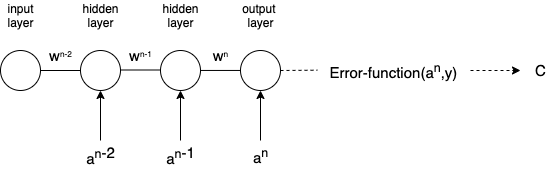
\includegraphics[scale=0.4]{latex/imgs/simplebackprop.png}
  \caption{simple neural network}\label{Baseline:before}
\end{figure}


\noindent
For a fully connected network which has more neurons per layer, the same idea can be applied. Having a neural network like the one seen in figure(14). For any neuron $i \in \{1,2,...,k\}$ in layer (n-1), and any neuron $j \in \{1,2,...,t\}$ in layer n, the impact $w_{ji}$ has on the cost is calculated by: \\

\begin{align}
\frac{\partial C}{\partial w_{ji}^n} =\frac{\partial z_j^n}{\partial w_{ji}^n}\frac{\partial a_j^n}{\partial z_j^n}\frac{\partial C}{  \partial a_j^n}
\end{align}

\noindent
Now since each neruon impact multiple neurons, which each impacts the cost, the impact of how much the activation function impacts the cost is calculated, like:

\begin{align}
\frac{\partial C}{\partial a^{n-1}_k} = \sum^t_{j=1} \frac{\partial z_j^n}{\partial a_k^{n-1}}\frac{\partial a_j^n}{\partial z_j^n}\frac{\partial C}{  \partial a_j^n}
\end{align}

\begin{figure}[!ht]
  \centering
  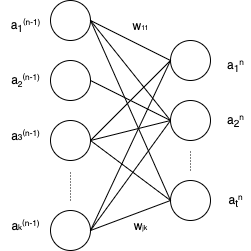
\includegraphics[scale=0.4]{latex/imgs/multibackprop.png}
  \caption{More complex neural network}\label{Baseline:before}
\end{figure}
